\documentclass[margin=0.5mm]{standalone}
%\documentclass[]{article}
\usepackage{lmodern}
\usepackage[utf8]{inputenc}
\usepackage[T1]{fontenc}
\usepackage{pgfplots}
\usepackage{pgfplotstable}

\pgfplotsset{width=\textwidth}

\begin{document}

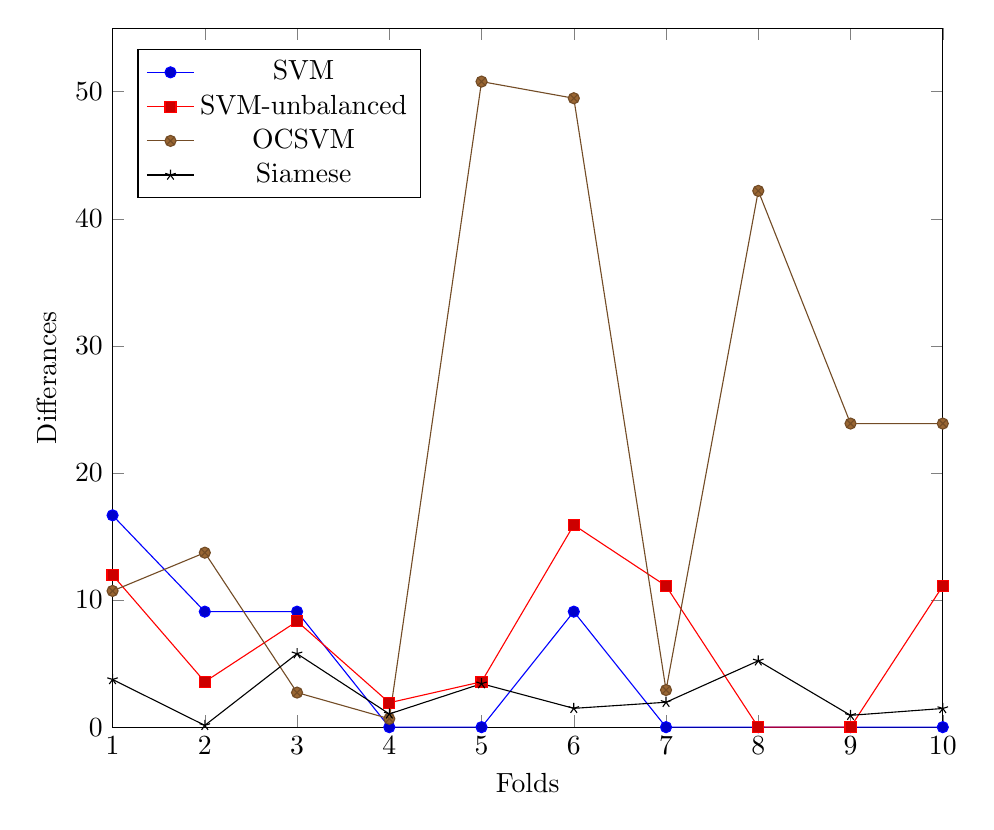
\begin{tikzpicture}
	\begin{axis}[%
	xlabel=Folds,
	ylabel= Differances,
	xmin=1,xmax=10, ymin=0, ymax=55, % <-- added here to preserve view
	legend pos=north west,
	]
		 \addplot coordinates
		{(1,16.67) (2,09.09) (3,09.09) (4,00.00) (5,00) (6,09.09) (7,00.00) (8,00.00) (9,00) (10,00) };
		\addlegendentry{SVM}
		\addplot coordinates
		{(1,11.97) (2,03.57) (3,08.33) (4,01.92) (5,03.57) (6,15.91) (7,11.11) (8,0) (9,0) (10,11.11) };
		\addlegendentry{SVM-unbalanced}
		\addplot coordinates
		{(1,10.72) (2,13.73) (3,02.72) (4,00.66) (5,50.80) (6,49.49) (7,02.92) (8,42.20) (9,23.89) (10,23.89) };
		\addlegendentry{OCSVM}
		\addplot coordinates
		{(1,03.75) (2,00.14) (3,05.78) (4,01.04) (5,03.42) (6,01.48) (7,01.96) (8,05.22) (9,00.93) (10,01.47) };
		\addlegendentry{Siamese}
	\end{axis}
\end{tikzpicture}

\end{document}